% http://www.miccai2013.org/submission_guideline.html
\documentclass{llncs}

\usepackage{amsmath}
\usepackage{makeidx}
\usepackage[pdftex]{graphicx}

\def\wrt{w.\,r.\,t.}
\def\eg{e.\,g.}
\def\ie{i.\,e.}
\def\Dash{\nobreak\,---\penalty-500\,}

%%% Comments
\usepackage{color}
\newcommand{\TG}[1]{{\color{blue}\textbf{TG: #1}}}
\newcommand{\CD}[1]{{\color{green}\textbf{CD: #1}}}
\newcommand{\IP}[1]{{\color{cyan}\textbf{IP: #1}}}
\newcommand{\TODO}[1]{{\color{red}\textbf{TODO: #1}}}
%%%

\renewcommand{\Vec}[1]{\mathbf{#1}}
\newcommand{\Mat}[1]{\mathbf{#1}}

\begin{document}
%
%\frontmatter          % for the preliminaries
%
\mainmatter              % start of the contributions
%
\title{Complete Real-Time Liver Model including Glisson Capsule, Vascular Network and Parenchyma}
%
\titlerunning{Complete Liver Model}  % abbreviated title (for running head)
%                                     also used for the TOC unless
%                                     \toctitle is used
%
\author{Anonymous}
%\author{%
%Tom\'a\v{s} Golembiovsk\'y\inst{1,2} \and%
%Igor Peterl\'ik\inst{3} \and%
%Christian Duriez\inst{2} \and%
%Stephan\'e Cotin\inst{2,3}%
%}
%
%\authorrunning{Tom\'a\vs Golembiovsk\'y et al.} % abbreviated author list (for running head)
%
%\institute{%
%Faculty of Informatics, Masaryk University, Brno, Czech Republic\and%
%INRIA Lille -- Nord, France\and%
%IHU, Strasbourg, France%
%}
%
\maketitle

\begin{abstract}
This work provides a complete physical model for the deformations of the liver with its three constituents: parenchyma, vessels and the Glisson's capsule.
Some recent experimental results \cite{Ahn2010} have shown that there is a significant difference of stiffness between the Glisson's capsule and the parenchyma. 
Moreover, it has been observed that the capsule plays an important role for the deformation at the local level \cite{Hollenstein2006}.
However, the Glisson's capsule is very thin and its influence for the global deformations of the liver was never highlighted.
In this work, we propose to use a membrane FEM model for the capsule, that is coupled with a vascularized model of the liver.
We show that the approach is able to reproduce the deformations observed at the local level.
Additionally, we show, by simulating natural global deformations of the liver observed on real images (due to gravity), that the results have important differences with and without the capsule.

\keywords{liver, Glisson's capsule, vascular network, deformation modeling, membrane}
\end{abstract}

\section{Introduction} 
\IP{I think we should provide some introductory motivation and broader context of the reasarch. I tried this:}

According to the statistics, nearly 100,000 European citizens die of cirrhosis or liver cancer each year. 
Although new methods such as radio-frequency ablation or cryo-ablation used in interventional radiology 
represent promising improvements, surgery remains the option that offers the foremost success rate against these pathologies. 
Nevertheless, surgery is not always performed due to several limitations, in particular the determination 
of accurate eligibility criteria for the patient. 
In this context, pre-operational planning becomes a crucial task having a significant impact on the treatment. 

Computer-aided physics-based medical simulation has proven to be an extremely useful technique in the area of medical training. 
Nevertheless, whereas generic models are usually required in training simulators, accurate patient-specific modelling
becomes necessary as soon as computer simulation is to be employed in the pre-operative planning. At the same time, 
interactivity of such models  remains an important aspect, requiring real-time simulation which is often difficult to 
achieve given the complexity of soft tissues. 

In case of human liver, the task of real-time accurate modeling is challenging, mainly because of the complex structure 
of this organ composed of three main constituents: \emph{parenchyma}, \emph{vascular networks} and \emph{Glisson's capsule}.
The parenchyma has certainly been the most studied component of the liver; today the researchers agree on hyperelastic 
properties of the tissue, for which the mechanical parameters have been reported for example in~\cite{Kerdok2006,Gao2009}. 
Several methods have been proposed to model the hyperelastic behaviour at real-time rates, such as multiplicative Jacobian decomposition
introduced in~\cite{Marchesseau2010}.

The mechanical importance of the vascular structures in liver is studied in~\cite{Peterlik2012}. It shows that the 
influence of vessels on the mechanical behaviour of the liver is significant, mainly if large deformations occur. 
Since detailed modeling of the vessels would be extremely costly (mainly because of the thickness of the vessel wall 
being less than 250\,{$\mu$}m), the authors propose a composite model allowing for real-time simulation of entire liver
with two vascular trees corresponding to portal and hepatic veins.

Rather a small number of studies have been conducted on the last liver constituent, the  Glisson's capsule.
Quantitative results of experiments on a porcine liver have been published in~\cite{Umale2013}. The measurements indicate that although being very 
thin (10--20$\mu m$), the capsule shows to be stiff in tensile tests mainly if compared to the parenchyma: the Young's modulus of the capsule (reported as $8.22\pm3.42$\,MPa) exceeds the values for the parenchyma by three orders of magnitude.
This suggests that the mechanical influence of the membrane on the liver behaviour is significant.

In~\cite{Hollenstein2006}, a local influence of the capsule has been measured using a special aspiration device. The study was then repeated 
in vivo on human patients during the operation, confirming the mechanical importance of the membrane~\cite{Ahn2010,Nava2008}.
To our best knowledge, no attempt has been made to demonstrate the role of the Glisson's capsule on the global behaviour of 
the liver, mainly if large deformations of the organ take place.

The main contribution of the paper is twofold: first, we present an efficient real-time model of the liver, taking into account 
the parenchyma, vascularization and Glisson's capsule. The model is based on three different finite element representations for each constituent,
linked together via mechanical coupling. We show that the model mimics the \emph{local} experiments described in~\cite{Hollenstein2006}.
 
Second, we use the complete model of the liver to demonstrate the \emph{global} influence of the Glisson's
capsule via simulation: using a specific model of a porcine liver built from CT contrast-enhanced data, we show that there is a significant 
difference in the response of the model with and without the capsule in case when the liver undergoes large deformations. 

The paper is organized as follows: \TODO{paper organization}.


%Medical simulation is expected to play an integral part in many aspects of
%medical practice. From diagnosis, through planning or training to computer
%assisted intervention.
%Medical training application, like the ones for training laparoscopic
%surgery, have to operate in real-time and a good medical model has to be
%simple yet efficient to be really usable in this environment.
%
%Liver is largest internal organ formed mostly by a soft tissue (parenchyma)
%that is hyper-elastic and also visco-elastic. The parenchyma is interwoven
%by dense vascular network, this tree-like tubular structure is stiffer then
%the parenchyma. Finally the parenchyma is covered by very stiff collagenous
%membrane that preserves the integrity of the organ.
%
%Strangely, most of the work on liver modelling only considers the
%parenchyma and model the liver as single homogeneous object \TG{Refs}.
%Only recently
%Peterl\'{i}k et al. \cite{Peterlik2012} showed the importance of the vascular
%structures on the liver deformation.
%
%Another overlooked component is the Glisson's capsule.
%Biomechanical measurements report that the capsule has very small
%thickness (approx. 20 $\mu$m for porcine liver \cite{Umale2011}).
%On the other hand it has in three orders of magnitude higher stiffness than
%the parenchyma.
%Because of this it plays an important role in local
%deformations of the liver \cite{Ahn2010,Hollenstein2006}.
%It was reported that evaluation of the liver as a homogeneous material
%without capsule can lead to overestimation of local deformations up to the factor of 3
%\cite{Hollenstein2006}.
%
%While the influence on local deformation was reported, no experimental
%results show whether the capsule also plays an important role in global
%deformations of the liver. We propose a composite model that models the
%capsule with membrane FEM elements. We show that the model is able to
%simulate expected local behaviour reported in literature. Further more we
%show that the capsule plays also an important role in the deformation on
%global scale.

\TG{summary of following sections.}

%}}}


\section{Model} %{{{

In this section we describe the construction of our composite model
being composed of three main components: tetrahedral FE model of the 
parenchyma, Tymoshenko-beam model for the vascular structures and finally 
triangular membrane elements used for the capsule.

\subsection{Parenchyma and Vascularization} %{{{

It is known that the parenchyma exhibits non-linear viscoelastic behaviour \cite{Marchesseau2010}.
However, as we are mainly interested in the static equilibrium, we do not model the time-dependent
phenomena related to viscosity.

%However, we employ simpler corotational model as we are not so much
%interested in time-dependent behaviour but rather in static equilibrium
%under certain conditions.
%We also rely on the vascularized model of the parenchyma proposed by
%Peterl\'{i}k et al. \cite{Peterlik2012}.

The parenchyma is modeled using corotational finite elements~\cite{Felippa2005}.
While relying on linear stress-strain relationship, it allows for large displacements including rotations. 
While in the full non-linear formulation, the stiffness matrix relates the forces a $\Vec{f}$ and 
displacements $\Vec{u}$ as $\Vec{f} = \Mat{K}(\Vec{u})$, the corotational model 
requires the stiffness matrix $\Mat{K}_0$ of the system be computed only once before the simulation begins. 
Then, in each step, the motion of each element $e$ is decomposed into rigid rotation $\Mat{R}^e$ and local deformation. 
The rotations are then used to update each local element stiffness matrix as $\Mat{R}\Mat{K}_0\Mat{R}^{\top}$
whereas the deformations are used to compute the linear strain in the local corotational frame.
%The stiffness matrix $\Mat{K}$ can be expressed in terms of the deformation
%$u$ and the force as $\Vec{f} = \Mat{K}(\Vec{u}) \Vec{u}$. 
%Where the
%components of $\Mat{K}$ depend on the orientation of each element in the
%current simulation step.
%the rigid component is  
% The corotational
%formulation allows us to deal with geometrical non-linearities but still
%relies on linear stress-strain relationship. Thus rotations and large
%deformations are modelled correctly. 
%In the corotational formulation the deformation
%of each element is expressed in the local frame of reference. 
There are several ways of computing the corotational frame for elements; we rely on
the geometrical method proposed in \cite{Nesme2005}.
% NOTE: This description of corotational method is very simplified and could be extended.

The model of the vascularization is based on linear beams 
with local frames of reference; in many aspects it's similar to the
corotational formulation described above~\cite{Duriez2006}. As such the model also handles geometric
non-linearities in the deformation. Through a specification of cross section and moments of inertia, 
the model can account for the specific properties of the blood vessels. 

The beam-based model of vessels is mechanically coupled to the parenchyma as described in~\cite{Peterlik2012}. 
The coupling assumes that there is no relative motion between the vessels and surrounding parenchyma. 
%The proposed model assumes no relative
%motion of vessels to the parenchyma. Segmented vascular network is
%discretized into the set of linear elements that are then projected into
%the tetrahedral mesh of the parenchyma. 
During the simulation, the nodes of linked beams are first displaced and rotated according to the actual motion of associated tetrahedra. 
As the deformation of beams results in mechanical response represented by forces and torques, these are propagated back to 
the tetrahedral FE model. 

%a displacement of tetrahedral nodes are mapped  forces and torques resulting from the deformations of vessels by parenchyma are
%computed and propagated back onto the tetrahedral mesh.

%}}}

\subsection{Glisson's Capsule} %{{{

The thickness of the Glisson's capsule is relatively small. Umale et al.
\cite{Umale2011} reported for porcine liver values in range of 10-20
$\mu$m.
It is not possible to model such thin structure with classical tetrahedral
elements. Modeling this non-homogeneous volumetric object would require a
dense mesh to avoid numerical instabilities and would significantly
violate the speed requirements imposed on medical simulators.
Instead modeling the capsule with two-dimensional elements that abstract from the
thickness in the third dimension seems
as a natural choice. Mechanics provides this a FE tool in the form of membranes
and shells. Based on the small thickness (compared to the surface area) we also
assume negligible bending forces and propose a model based on membrane
elements. 
To maintain simplicity of the composite model we choose simple triangular
elements with constant strain (CST).

The computation of elastic stiffness matrix follows the common derivation

\begin{eqnarray}
  \Mat{K}^m & = \int_V \Mat{B}^T \Mat{E} \Mat{B} dV     \label{mem1} \\
            & = h \int_A \Mat{B}^T \Mat{E} \Mat{B} dA   \label{mem2} \\
            & = h A \Mat{B}^T \Mat{E} \Mat{B}           \label{mem3}
\end{eqnarray}

where $\Mat{B}$ is the strain-displacement matrix, $\Mat{E}$ the material
matrix, $h$ is the thickness and $A$ area of the element. In the previous
\eqref{mem2} follows from the fact that we assume constant thickness of the
element and \eqref{mem3} follows from the fact that the strain-displacement
matrix is in our case constant. The strain-displacement matrix for the CST
element can be expressed as:

\begin{equation}
  \Mat{B} = \frac{1}{2A} \begin{bmatrix}
    y_{23} & 0      & y_{31} & 0      & y_{12} & 0 \\
         0 & x_{32} & 0      & x_{13} & 0      & x_{21} \\
    x_{32} & y_{23} & x_{13} & y_{31} & x_{21} & y_{12}
  \end{bmatrix}
\end{equation}

The values $x_{ij} = x_i - x_j$ and $y_{ij} = y_i - y_j$ are computed from
the $x$ or $y$ coordinates of the nodes $i,j$ of the triangular element.
The reader can reffer to the respective literature for more thorough
description \cite{Felippa2003}.

We again use linear elastic material and employ the corotational formulation
for the triangular elements.

%}}}

\subsection{Coupling Between Capsule and Parenchyma} %{{{

The literature reports high cohesion between capsule and parenchyma.
Based on this
property we may assume no relative motion of the capsule to the parenchyma.
While in general we could use arbitrary surface mesh for a capsule we use
the fact that the parenchyma is modeled by tetrahedral elements which have
triangular faces. Because the boundary of the volumetric mesh is already
triangulated, we only extract the boundary triangles which we use for the
model of capsule.

Using directly the boundary of the tetrahedral mesh does not only solve the
problem of obtaining the surface mesh, but has one more advantage. Nodes
of the triangular mesh overlap with nodes of the tetrahedral mesh and we do
not have to project nodes of triangular mesh onto the tetrahedra. More over,
the stiffness matrices for capsule and parenchyma are easily assembled
together and solved as one system.

\CD{The following may appear as "trivial"... maybe we can remove this part at the end if we need space} 
Without the loss of generality we can assume the tetrahedron consists of
nodes $p_1, p_2, p_3$ and $p_4$ and the boundary triangle has nodes $p_1, p_2$
and $p_3$. We can reorder the degrees of freedom so that the stiffness
matrix $\Mat{K}^t$ for the tetrahedron can be written as:

\begin{equation}
  \Mat{K}^t = \left[\begin{array}{c|c}
      \Mat{K}^t_{1-3,1-3} & \Mat{K}^t_{1-3,4} \\
      \hline
      \Mat{K}^t_{4,1-3} & \Mat{K}^t_{4,4} \\
  \end{array}\right]
\end{equation}

Then the assembled stiffness matrix for the element is:

\begin{equation}
  \Mat{K} = \left[\begin{array}{c|c}
      \Mat{K}^t_{1-3,1-3} & \Mat{K}^t_{1-3,4} \\
      \hline
      \Mat{K}^t_{4,1-3} & \Mat{K}^t_{4,4} \\
  \end{array}\right]
  +
  \left[\begin{array}{c|c}
      \Mat{K}^m & 0 \\
      \hline
      0 & 0 \\
  \end{array}\right]
\end{equation}

Where $\Mat{K}^m$ is the stiffness matrix of the triangular membrane.
The resulting
system of linear equations is then solved by direct LDL solver.

%}}}

%}}}


\section{Experiments} %{{{

To evaluate the model it was implemented in the
SOFA\footnote{www.sofa-framework.org} framework and a set of
numerical simulations was performed. First local deformations were compared to the
results reported in literature to validate the method.

To show that, despite its very small thickness, the membrane cannot be
neglected even in the context of global deformations and its overall
stiffness plays an important role, the model of
the complete liver was subjected to natural global deformations.

In the simulations we used material properties for a porcine liver as
reported by Umale \cite{Umale2013}. The
parenchyma was modeled with elastic modulus 1980~Pa and the capsule has
elastic modulus 8~MPa and thickness 20~$\mu$m.
\IP{OK, now we must decide what value we are going to use for the parenchyma, so it does not explode but it's somehow reasonable...)}
\TG{Right now I'm using 3500 Pa for parenchyma. I can even use higher
modulus, but not any smaller because we get large deformations and use of
corotational model might become questionable.}

\TG{values for blood vessels}

\IP{we have to also add some information how we got the models -- either we comment briefly in each subsection:
Local deformations: cube meshed in gmsh (graded mesh?), number of elements, etc...
Global deformations: contrast-enhanced CT data obtained via acquisition performed on a female pig; the 3D mesh created by a
semi-automatic segmentation using ITKSnap\footnote{www.itksnap.org}, then meshed using CGAL\footnote{www.cgal.org} \cite{Boltcheva2009} resulting in a mesh having 
NNN elements. The capsule modelled using the surface triangular elements extracted from the tetrahedra. The vascularization 
created from the segmentation of hepatic vein as described in~\cite{Peterlik2012}. The structured composed of MMM elements.}
\TG{Sure. Put it here or into the respective subsections? (cube: graded
  mesh created by gmsh with 2648 tetrahedra, 518 triangles for capsule
extracted from tetrahedral mesh.)}



\subsection{Local Deformations} %{{{

During the contact with an instrument (probe, needle insertion, sharp
instruments, \ldots) a specific deformation occurs in the near vicinity of
the instrument. This type of deformation may not necessarily induce the
deformation of the object as a whole and therefore can be considered as
local. Correct material properties are not only important for amount of the
displacement but play also a crucial role in capturing the correct area of
the deformation or its profile near the instrument.
\TG{Does it make sense this way? I can add an image. :)}

One example of such local deformation occurs during the aspiration test
when the response of liver to the negative pressure is measured.
Hollenstein et al. \cite{Hollenstein2006} observed that the Glisson's
capsule has non-negligible influence on response of the tissue and modeling
only the parenchyma leads to overestimation of the deformation. We
reproduced the test with our model and acquired similar results.

The aspiration device consists of a tube with 1 cm in diameter and is able
to control internal pressure in the tube. The test is performed by
attaching the tube to the tissue and measuring the tissue response. We
have set up a simulation in the spirit of this test. 
The simulation is performed with a 15x15x15 mm cube of liver tissue and tube
with 1 cm in diameter. The pressure of 3 kPa is simulated inside the tube.

Figure \ref{fig-aspiration} shows the profiles of cuts in the middle of the
test cube. It can be seen that the
deformation for the model without capsule is much larger. This is in good
agreement with the data obtained by Hollenstein et al.

\begin{figure}[htb]
  \centering
  \begin{tabular}{cc}
    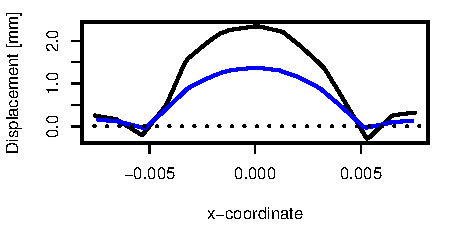
\includegraphics[width=3in]{aspiration.pdf} &
    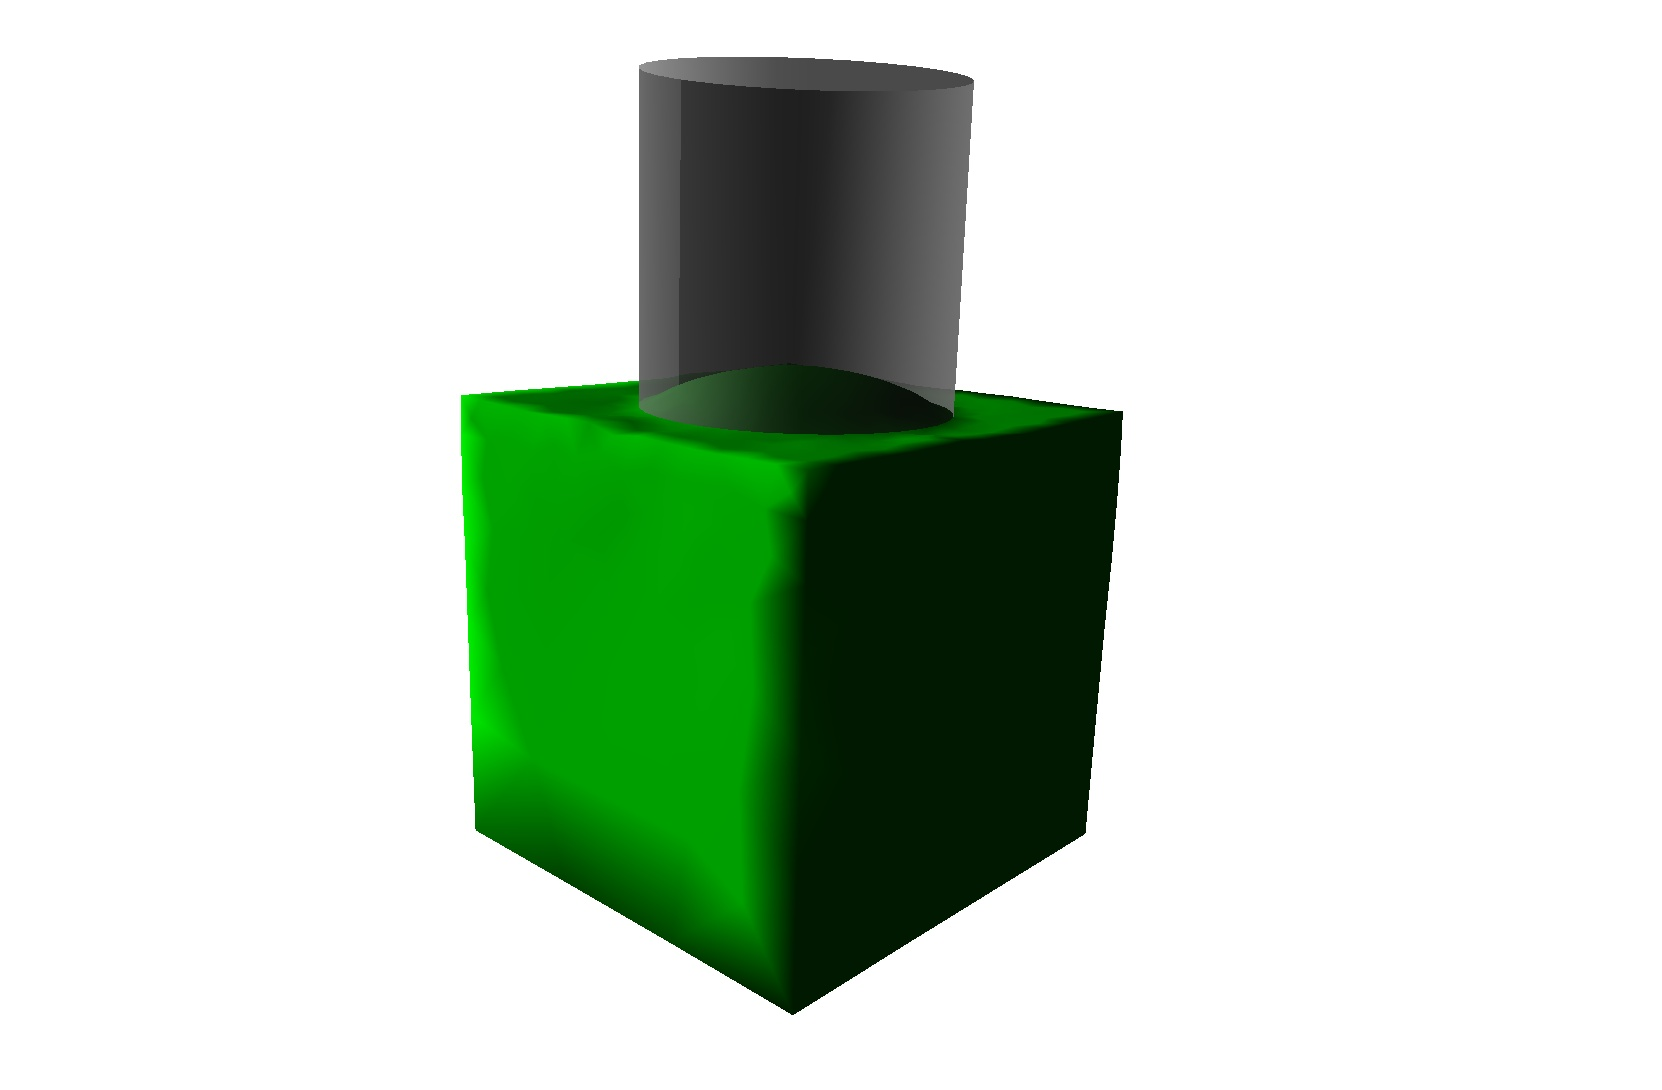
\includegraphics[height=1.5in]{aspiration.jpg}\\
    a) & b)
  \end{tabular}

  \caption{\label{fig-aspiration}Aspiration test: a) displacment profile
  with (blue) and without (black) the capsule; b) simulation scene}
\end{figure}


%}}}




\subsection{Global Deformations}
\CD{ Experiments demonstrate that capsule plays a role at local level, but still, maybe not so important to model the capsule for more global deformation...
+ What are the applications for modeling the global deformations of the liver (training and planning simulation, physics-based registration, augmented reality,)}


\TG{!!!}

%Test 1) Global deformation of liver under gravity
%  * show that there is a difference between simple homogeneous material
%    and material with capsule
%  * include blood vessels

\IP{Short overview, I'll put it together tomorrow morning and add some fancy images. I am not sure if we are going to mess up 
with gravity, it seems to me too much... We should rather focus only on this "registration-like" simulation (what about 
using term "elastic warping"??? and explain properly why we think it proves the capsule plays a role. My first shot:}

--we want to mimic a process takes place inside the pig such that it results in a natural deformation of the liver

--such a natural deformation happens when the position of the pig is changed from the flank to a supine position

--we performed a segmentation of both flank and supine and for some parts of the liver, displacements up to XXX\,cm  (I would say 3-4) 
were observed, which is enough given the size of the entire liver (18\,cm longest dimension)

--to induce the same deformation on the liver, we performed a process similar to deformation registration between the flank and supine 
data: we chosen a set of feature in flank and supine data such that each feature could be reliably located in both supine and flank 
data

--this set of features was extracted from the vascularization, since although the vascular tree is getting deformed together with the liver, 
the topology remains constant

--then we placed a linear spring to each feature location in the supine data, so it's attracted towards its flank position

--since the features were mapped to the elements via barycentric mapping, the entire model of the liver is being deformed, "elastically warped" from the 
supine to the flank position


--now the tricky part begins: we performed this process with models with and without the capsule; in each case we obtained 
a different resulting shape of liver

--additionally, we measured the forces needed to warp the liver in both cases: we obtained a difference summarized as.... ???


%}}}

\section{Conclusion} %{{{

A composite model for simulation of complete liver is presented in the
paper. The work of Peterlik et al. for vaskularized liver model was
extended by addig the capsule modeled with membrane FEM model mechanically
coupled with the parenchyma. To validate the model a simulation of local
deformations was performed and was found in an aggrement with the results
measured and published by Hollenstein et al.

While the influence of the capsule on local deformations was previously
studied in the literature, it's significance on the global scale
deformations of the liver remained unexplored. We have performed a set of
natural global deformations of the complete liver and shown that the
capsule, despite its small thickness, plays a significant role also in
global context.

%}}}

%
% ---- Bibliography ----
%

\bibliographystyle{splncs03}
\bibliography{bibdata}


\end{document}
% spell: setl spell spelllang=en spellfile=spelldict.en.utf-8.add
% vim:set et sw=2 tw=75 fdm=marker fdl=3 fdc=4 isk+=_,-:
